% Options for packages loaded elsewhere
\PassOptionsToPackage{unicode}{hyperref}
\PassOptionsToPackage{hyphens}{url}
%
\documentclass[
]{article}
\usepackage{amsmath,amssymb}
\usepackage{lmodern}
\usepackage{iftex}
\ifPDFTeX
  \usepackage[T1]{fontenc}
  \usepackage[utf8]{inputenc}
  \usepackage{textcomp} % provide euro and other symbols
\else % if luatex or xetex
  \usepackage{unicode-math}
  \defaultfontfeatures{Scale=MatchLowercase}
  \defaultfontfeatures[\rmfamily]{Ligatures=TeX,Scale=1}
\fi
% Use upquote if available, for straight quotes in verbatim environments
\IfFileExists{upquote.sty}{\usepackage{upquote}}{}
\IfFileExists{microtype.sty}{% use microtype if available
  \usepackage[]{microtype}
  \UseMicrotypeSet[protrusion]{basicmath} % disable protrusion for tt fonts
}{}
\makeatletter
\@ifundefined{KOMAClassName}{% if non-KOMA class
  \IfFileExists{parskip.sty}{%
    \usepackage{parskip}
  }{% else
    \setlength{\parindent}{0pt}
    \setlength{\parskip}{6pt plus 2pt minus 1pt}}
}{% if KOMA class
  \KOMAoptions{parskip=half}}
\makeatother
\usepackage{xcolor}
\usepackage[margin=1in]{geometry}
\usepackage{color}
\usepackage{fancyvrb}
\newcommand{\VerbBar}{|}
\newcommand{\VERB}{\Verb[commandchars=\\\{\}]}
\DefineVerbatimEnvironment{Highlighting}{Verbatim}{commandchars=\\\{\}}
% Add ',fontsize=\small' for more characters per line
\usepackage{framed}
\definecolor{shadecolor}{RGB}{248,248,248}
\newenvironment{Shaded}{\begin{snugshade}}{\end{snugshade}}
\newcommand{\AlertTok}[1]{\textcolor[rgb]{0.94,0.16,0.16}{#1}}
\newcommand{\AnnotationTok}[1]{\textcolor[rgb]{0.56,0.35,0.01}{\textbf{\textit{#1}}}}
\newcommand{\AttributeTok}[1]{\textcolor[rgb]{0.77,0.63,0.00}{#1}}
\newcommand{\BaseNTok}[1]{\textcolor[rgb]{0.00,0.00,0.81}{#1}}
\newcommand{\BuiltInTok}[1]{#1}
\newcommand{\CharTok}[1]{\textcolor[rgb]{0.31,0.60,0.02}{#1}}
\newcommand{\CommentTok}[1]{\textcolor[rgb]{0.56,0.35,0.01}{\textit{#1}}}
\newcommand{\CommentVarTok}[1]{\textcolor[rgb]{0.56,0.35,0.01}{\textbf{\textit{#1}}}}
\newcommand{\ConstantTok}[1]{\textcolor[rgb]{0.00,0.00,0.00}{#1}}
\newcommand{\ControlFlowTok}[1]{\textcolor[rgb]{0.13,0.29,0.53}{\textbf{#1}}}
\newcommand{\DataTypeTok}[1]{\textcolor[rgb]{0.13,0.29,0.53}{#1}}
\newcommand{\DecValTok}[1]{\textcolor[rgb]{0.00,0.00,0.81}{#1}}
\newcommand{\DocumentationTok}[1]{\textcolor[rgb]{0.56,0.35,0.01}{\textbf{\textit{#1}}}}
\newcommand{\ErrorTok}[1]{\textcolor[rgb]{0.64,0.00,0.00}{\textbf{#1}}}
\newcommand{\ExtensionTok}[1]{#1}
\newcommand{\FloatTok}[1]{\textcolor[rgb]{0.00,0.00,0.81}{#1}}
\newcommand{\FunctionTok}[1]{\textcolor[rgb]{0.00,0.00,0.00}{#1}}
\newcommand{\ImportTok}[1]{#1}
\newcommand{\InformationTok}[1]{\textcolor[rgb]{0.56,0.35,0.01}{\textbf{\textit{#1}}}}
\newcommand{\KeywordTok}[1]{\textcolor[rgb]{0.13,0.29,0.53}{\textbf{#1}}}
\newcommand{\NormalTok}[1]{#1}
\newcommand{\OperatorTok}[1]{\textcolor[rgb]{0.81,0.36,0.00}{\textbf{#1}}}
\newcommand{\OtherTok}[1]{\textcolor[rgb]{0.56,0.35,0.01}{#1}}
\newcommand{\PreprocessorTok}[1]{\textcolor[rgb]{0.56,0.35,0.01}{\textit{#1}}}
\newcommand{\RegionMarkerTok}[1]{#1}
\newcommand{\SpecialCharTok}[1]{\textcolor[rgb]{0.00,0.00,0.00}{#1}}
\newcommand{\SpecialStringTok}[1]{\textcolor[rgb]{0.31,0.60,0.02}{#1}}
\newcommand{\StringTok}[1]{\textcolor[rgb]{0.31,0.60,0.02}{#1}}
\newcommand{\VariableTok}[1]{\textcolor[rgb]{0.00,0.00,0.00}{#1}}
\newcommand{\VerbatimStringTok}[1]{\textcolor[rgb]{0.31,0.60,0.02}{#1}}
\newcommand{\WarningTok}[1]{\textcolor[rgb]{0.56,0.35,0.01}{\textbf{\textit{#1}}}}
\usepackage{graphicx}
\makeatletter
\def\maxwidth{\ifdim\Gin@nat@width>\linewidth\linewidth\else\Gin@nat@width\fi}
\def\maxheight{\ifdim\Gin@nat@height>\textheight\textheight\else\Gin@nat@height\fi}
\makeatother
% Scale images if necessary, so that they will not overflow the page
% margins by default, and it is still possible to overwrite the defaults
% using explicit options in \includegraphics[width, height, ...]{}
\setkeys{Gin}{width=\maxwidth,height=\maxheight,keepaspectratio}
% Set default figure placement to htbp
\makeatletter
\def\fps@figure{htbp}
\makeatother
\setlength{\emergencystretch}{3em} % prevent overfull lines
\providecommand{\tightlist}{%
  \setlength{\itemsep}{0pt}\setlength{\parskip}{0pt}}
\setcounter{secnumdepth}{-\maxdimen} % remove section numbering
\usepackage{booktabs}
\usepackage{longtable}
\usepackage{array}
\usepackage{multirow}
\usepackage{wrapfig}
\usepackage{float}
\usepackage{colortbl}
\usepackage{pdflscape}
\usepackage{tabu}
\usepackage{threeparttable}
\usepackage{threeparttablex}
\usepackage[normalem]{ulem}
\usepackage{makecell}
\usepackage{xcolor}
\ifLuaTeX
  \usepackage{selnolig}  % disable illegal ligatures
\fi
\IfFileExists{bookmark.sty}{\usepackage{bookmark}}{\usepackage{hyperref}}
\IfFileExists{xurl.sty}{\usepackage{xurl}}{} % add URL line breaks if available
\urlstyle{same} % disable monospaced font for URLs
\hypersetup{
  pdftitle={TSA Final Forecasting},
  pdfauthor={Yinan Ding, Jinxi Liu, Zhengqi Jiao},
  hidelinks,
  pdfcreator={LaTeX via pandoc}}

\title{TSA Final Forecasting}
\author{Yinan Ding, Jinxi Liu, Zhengqi Jiao}
\date{2023-04-11}

\begin{document}
\maketitle

\begin{Shaded}
\begin{Highlighting}[]
\CommentTok{\#Load/install required package here}
\FunctionTok{library}\NormalTok{(lubridate)}
\FunctionTok{library}\NormalTok{(ggplot2)}
\FunctionTok{library}\NormalTok{(forecast)  }
\FunctionTok{library}\NormalTok{(Kendall)}
\FunctionTok{library}\NormalTok{(tseries)}
\FunctionTok{library}\NormalTok{(outliers)}
\FunctionTok{library}\NormalTok{(tidyverse)}
\FunctionTok{library}\NormalTok{(smooth)}
\FunctionTok{library}\NormalTok{(kableExtra)}
\FunctionTok{library}\NormalTok{(dplyr)}
\FunctionTok{library}\NormalTok{(zoo)}
\end{Highlighting}
\end{Shaded}

\#\#Checking working directory

\begin{Shaded}
\begin{Highlighting}[]
\FunctionTok{getwd}\NormalTok{()}
\end{Highlighting}
\end{Shaded}

\begin{verbatim}
## [1] "C:/Users/estre/Desktop/Time-series/TSA-Final-Project"
\end{verbatim}

\#\#Import Data

\begin{Shaded}
\begin{Highlighting}[]
\NormalTok{hourlyprice.raw }\OtherTok{\textless{}{-}} \FunctionTok{read.csv}\NormalTok{(}\StringTok{"./Data/Day{-}Ahead\_Zonal\_Price\_NYC\_2010{-}2022.csv"}\NormalTok{,}\AttributeTok{stringsAsFactors =} \ConstantTok{FALSE}\NormalTok{) }\CommentTok{\# hourly LBMP of NYC from January 2010 to December 2022}
\CommentTok{\#hourlyload.raw \textless{}{-} read.csv("./Data/NYC Load\_Forecast\_2018{-}2022.csv",stringsAsFactors = FALSE) \# hourly LBMP of NYC from January 2018 to December 2022}
\CommentTok{\#NGprice.raw \textless{}{-} read.csv("./Data/Henry\_Hub\_Natural\_Gas\_Spot\_Price.csv",stringsAsFactors = FALSE) \# Daily NG Price from January 2018 to December 2022}
\CommentTok{\#REgeneration.raw \textless{}{-} read.csv("./Data/Monthly Renewable Generation\_2018{-}2022.csv",stringsAsFactors = FALSE) \# RE generation from January 2008 to December 2022}

\FunctionTok{head}\NormalTok{(hourlyprice.raw, }\DecValTok{10}\NormalTok{)}
\end{Highlighting}
\end{Shaded}

\begin{verbatim}
##             date Eastern.Date.Hour.Time.Zone Zone.Name Zone.PTID DAM.Zonal.LBMP
## 1  1/1/2010 0:00                         EST    N.Y.C.     61761          47.58
## 2  1/1/2010 1:00                         EST    N.Y.C.     61761          46.04
## 3  1/1/2010 2:00                         EST    N.Y.C.     61761          40.96
## 4  1/1/2010 3:00                         EST    N.Y.C.     61761          43.07
## 5  1/1/2010 4:00                         EST    N.Y.C.     61761          43.59
## 6  1/1/2010 5:00                         EST    N.Y.C.     61761          42.50
## 7  1/1/2010 6:00                         EST    N.Y.C.     61761          44.19
## 8  1/1/2010 7:00                         EST    N.Y.C.     61761          43.99
## 9  1/1/2010 8:00                         EST    N.Y.C.     61761          50.81
## 10 1/1/2010 9:00                         EST    N.Y.C.     61761          56.17
##    DAM.Zonal.Losses DAM.Zonal.Congestion
## 1              3.22               -10.45
## 2              2.91                -9.28
## 3              2.84                -4.31
## 4              2.56                -7.71
## 5              2.74                -7.08
## 6              2.91                -5.74
## 7              2.88                -7.81
## 8              2.80                -8.24
## 9              2.94               -14.02
## 10             3.12               -19.13
\end{verbatim}

\begin{Shaded}
\begin{Highlighting}[]
\CommentTok{\#head(hourlyload.raw, 10)}
\end{Highlighting}
\end{Shaded}

\#\#Data Wrangling - hourly to daily

\begin{Shaded}
\begin{Highlighting}[]
\FunctionTok{class}\NormalTok{(hourlyprice.raw}\SpecialCharTok{$}\NormalTok{Date)}
\end{Highlighting}
\end{Shaded}

\begin{verbatim}
## [1] "NULL"
\end{verbatim}

\begin{Shaded}
\begin{Highlighting}[]
\FunctionTok{class}\NormalTok{(hourlyprice.raw}\SpecialCharTok{$}\NormalTok{DAM.Zonal.LBMP)}
\end{Highlighting}
\end{Shaded}

\begin{verbatim}
## [1] "numeric"
\end{verbatim}

\begin{Shaded}
\begin{Highlighting}[]
\NormalTok{hourlyprice.raw }\OtherTok{\textless{}{-}}\NormalTok{ hourlyprice.raw }\SpecialCharTok{\%\textgreater{}\%}
  \FunctionTok{separate}\NormalTok{(date, }\AttributeTok{into =} \FunctionTok{c}\NormalTok{(}\StringTok{"date"}\NormalTok{, }\StringTok{"time"}\NormalTok{), }\AttributeTok{sep =} \StringTok{" "}\NormalTok{)}
\end{Highlighting}
\end{Shaded}

\begin{verbatim}
## Warning: Expected 2 pieces. Missing pieces filled with `NA` in 43824 rows
## [70129, 70130, 70131, 70132, 70133, 70134, 70135, 70136, 70137, 70138, 70139,
## 70140, 70141, 70142, 70143, 70144, 70145, 70146, 70147, 70148, ...].
\end{verbatim}

\begin{Shaded}
\begin{Highlighting}[]
\NormalTok{hourlyprice }\OtherTok{\textless{}{-}}\NormalTok{ hourlyprice.raw }\SpecialCharTok{\%\textgreater{}\%}
  \FunctionTok{select}\NormalTok{(date,DAM.Zonal.LBMP) }\SpecialCharTok{\%\textgreater{}\%}
  \FunctionTok{rename}\NormalTok{(}\AttributeTok{Price =}\NormalTok{ DAM.Zonal.LBMP)}

\NormalTok{hourlyprice.raw}\SpecialCharTok{$}\NormalTok{date }\OtherTok{\textless{}{-}} \FunctionTok{as.Date}\NormalTok{(hourlyprice.raw}\SpecialCharTok{$}\NormalTok{date,}\AttributeTok{format =} \StringTok{"\%m/\%d/\%Y"}\NormalTok{)}
  
\NormalTok{dailyprice }\OtherTok{\textless{}{-}}\NormalTok{ hourlyprice }\SpecialCharTok{\%\textgreater{}\%}
  \FunctionTok{filter}\NormalTok{( }\SpecialCharTok{!}\FunctionTok{is.na}\NormalTok{(hourlyprice}\SpecialCharTok{$}\NormalTok{Price)) }\SpecialCharTok{\%\textgreater{}\%} 
  \FunctionTok{group\_by}\NormalTok{(date) }\SpecialCharTok{\%\textgreater{}\%} 
  \FunctionTok{summarise}\NormalTok{(}\AttributeTok{daily\_mean\_price =} \FunctionTok{mean}\NormalTok{(Price))}
  \CommentTok{\# slice(1:(n() {-} 1))}
            

\NormalTok{dailyprice.ts }\OtherTok{\textless{}{-}} \FunctionTok{msts}\NormalTok{(dailyprice}\SpecialCharTok{$}\NormalTok{daily\_mean\_price,}
                      \AttributeTok{seasonal.periods =} \FunctionTok{c}\NormalTok{(}\DecValTok{7}\NormalTok{,}\FloatTok{365.25}\NormalTok{),}
                      \AttributeTok{start =} \FunctionTok{c}\NormalTok{(}\DecValTok{2010}\NormalTok{,}\DecValTok{1}\NormalTok{,}\DecValTok{1}\NormalTok{)) }
\CommentTok{\# hourlyload.raw \textless{}{-} hourlyload.raw \%\textgreater{}\%}
\CommentTok{\#   separate(Eastern.Date.Hour  , into = c("date", "time"), sep = " ") \%\textgreater{}\%}
\CommentTok{\#   separate(time, into = c("hour", "minute"), sep = ":")}
\CommentTok{\# }
\CommentTok{\# hourlyload \textless{}{-} hourlyload.raw \%\textgreater{}\%}
\CommentTok{\#   select(date,hour,DAM.Forecast.Load) \%\textgreater{}\%}
\CommentTok{\#   rename(Demand = DAM.Forecast.Load)}
\CommentTok{\#   }
\CommentTok{\#   }
\CommentTok{\# dailyload \textless{}{-} hourlyload \%\textgreater{}\%}
\CommentTok{\#   filter(!is.na(hourlyload$Demand)) \%\textgreater{}\% }
\CommentTok{\#   group\_by(date) \%\textgreater{}\% \# here we left column with minutes out}
\CommentTok{\#   summarise( daily\_mean\_load = mean(Demand))\%\textgreater{}\%}
\CommentTok{\#   slice(1:(n() {-} 1))}
\CommentTok{\# }
\CommentTok{\# class(dailyload$date)}
\CommentTok{\# dailyload$date \textless{}{-} as.Date(dailyload$date,format = "\%m/\%d/\%Y")}
\CommentTok{\# }
\CommentTok{\# str(dailyload)}

\FunctionTok{autoplot}\NormalTok{(dailyprice.ts)            }
\end{Highlighting}
\end{Shaded}

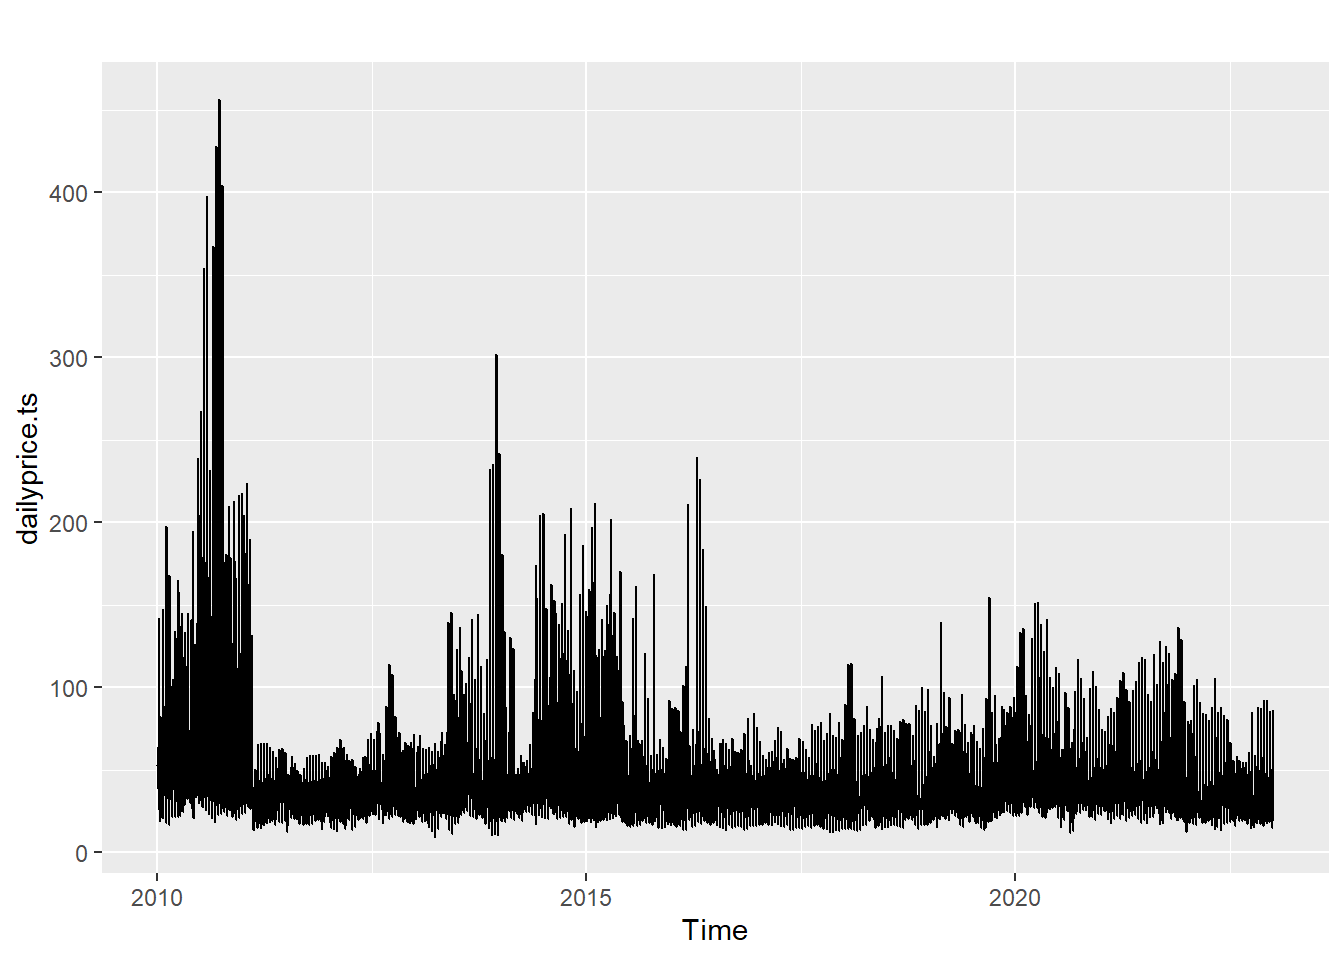
\includegraphics{TSA_Final_files/figure-latex/unnamed-chunk-2-1.pdf}

\begin{Shaded}
\begin{Highlighting}[]
\CommentTok{\# ggplot(dailyload, aes(x=date,y=daily\_mean\_load)) +}
\CommentTok{\#   geom\_line() +}
\CommentTok{\#   ggtitle("Average Daily Electricity Load in NYC from 2018 to 2022")+}
\CommentTok{\#   ylab("megawatthours")}
\end{Highlighting}
\end{Shaded}

\hypertarget{ng-fix-missing-dates}{%
\subsection{NG fix missing dates}\label{ng-fix-missing-dates}}

\begin{Shaded}
\begin{Highlighting}[]
\CommentTok{\# NGprice.raw$Day \textless{}{-}as.Date(NGprice.raw$Day,format = "\%m/\%d/\%Y")}
\CommentTok{\# \# Create a sequence of dates from the minimum to maximum date in the dataset}
\CommentTok{\# date\_seq \textless{}{-} data.frame(Day = seq(min(NGprice.raw$Day), max(NGprice.raw$Day), by = "day"))}
\CommentTok{\# }
\CommentTok{\# library(dplyr)}
\CommentTok{\# \# Merge the sequence of dates with the original dataset using a left join}
\CommentTok{\# complete\_data \textless{}{-} left\_join(date\_seq, NGprice.raw, by = "Day")}
\CommentTok{\# }
\CommentTok{\# \# Create a zoo object from the \textquotesingle{}value\textquotesingle{} column of the complete dataset}
\CommentTok{\# zoo\_data \textless{}{-} zoo(complete\_data$Natural.Gas.Spot.Price.Dollars.per.Million.Btu)}
\CommentTok{\# }
\CommentTok{\# \# Fill the missing values with the average of the previous day and the next day}
\CommentTok{\# zoo\_data\_filled \textless{}{-} na.approx(zoo\_data)}
\CommentTok{\# }
\CommentTok{\# \# Convert the filled zoo object back to a data frame}
\CommentTok{\# NGprice.fixed \textless{}{-} data.frame(Date = complete\_data$Day, value = coredata(zoo\_data\_filled))}
\CommentTok{\# }
\CommentTok{\# ggplot(NGprice.fixed, aes(x=Date,y=value)) +}
\CommentTok{\#   geom\_line() +}
\CommentTok{\#   ggtitle("Daily Natural Gas Spot Price from 2018 to 2022")+}
\CommentTok{\#   ylab("Dollars per Million Btu")}
\end{Highlighting}
\end{Shaded}

\#\#Data Wrangling - daily to monthly

\begin{Shaded}
\begin{Highlighting}[]
\CommentTok{\# NGprice.daily \textless{}{-} NGprice.fixed \%\textgreater{}\%}
\CommentTok{\#   rename(Price = value)}
\CommentTok{\# NGprice.daily$Date \textless{}{-}as.Date(NGprice.daily$Date,format = "\%m/\%d/\%Y")}
\CommentTok{\# }
\CommentTok{\# }
\CommentTok{\# \# Group the data by month and calculate the average price for each month}
\CommentTok{\# NGprice.monthly \textless{}{-} NGprice.daily \%\textgreater{}\%}
\CommentTok{\#   mutate(month = format(Date, "\%Y{-}\%m")) \%\textgreater{}\%}
\CommentTok{\#   group\_by(month) \%\textgreater{}\%}
\CommentTok{\#   summarise(avg\_price = mean(Price))}
\CommentTok{\# }
\CommentTok{\# }
\CommentTok{\# Monthlyprice \textless{}{-} dailyprice \%\textgreater{}\%}
\CommentTok{\#   mutate(month = format(date, "\%Y{-}\%m")) \%\textgreater{}\%}
\CommentTok{\#   group\_by(month) \%\textgreater{}\%}
\CommentTok{\#   summarise(monthly\_price = mean(daily\_mean\_price))}
\CommentTok{\# }
\CommentTok{\# Monthlyload \textless{}{-} dailyload \%\textgreater{}\%}
\CommentTok{\#   mutate(month = format(date, "\%Y{-}\%m")) \%\textgreater{}\%}
\CommentTok{\#   group\_by(month) \%\textgreater{}\%}
\CommentTok{\#   summarise(monthly\_load = mean(daily\_mean\_load))}
\CommentTok{\# }
\CommentTok{\# REgeneration.monthly \textless{}{-} REgeneration.raw \%\textgreater{}\% }
\CommentTok{\#   select(Total) \%\textgreater{}\%}
\CommentTok{\#   rename(REgeneration\_all = Total)}
\CommentTok{\# }
\CommentTok{\# start\_date \textless{}{-} as.Date("2018{-}01{-}01")}
\CommentTok{\# end\_date \textless{}{-} as.Date("2022{-}12{-}01")}
\CommentTok{\# monthly\_dates \textless{}{-} seq(start\_date, end\_date, by = "month")}
\CommentTok{\# }
\CommentTok{\# REgeneration.monthly \textless{}{-} REgeneration.monthly \%\textgreater{}\% }
\CommentTok{\#   mutate(date = monthly\_dates)}
\CommentTok{\# }
\CommentTok{\# ggplot(REgeneration.monthly, aes(x=date,y=REgeneration\_all)) +}
\CommentTok{\#   geom\_line() +}
\CommentTok{\#   ggtitle("Monthly REgeneration from 2018 to 2023")+}
\CommentTok{\#   ylab("Dollars per Million Btu")}
\end{Highlighting}
\end{Shaded}

\#\#Correlation Test

\begin{Shaded}
\begin{Highlighting}[]
\CommentTok{\# correlation.df \textless{}{-} data.frame(Monthlyprice$monthly\_price,REgeneration.monthly$REgeneration\_all, NGprice.monthly$avg\_price,Monthlyload$monthly\_load)}
\CommentTok{\# }
\CommentTok{\# correlation.df \textless{}{-} correlation.df \%\textgreater{}\%}
\CommentTok{\#   rename(Eprice=Monthlyprice.monthly\_price,NGprice=NGprice.monthly.avg\_price,REgeneration=REgeneration.monthly.REgeneration\_all,Eload=Monthlyload.monthly\_load)}
\CommentTok{\# }
\CommentTok{\# correlation.model \textless{}{-} lm(data = correlation.df, Eprice\textasciitilde{}NGprice+REgeneration+Eload)}
\CommentTok{\# summary(correlation.model)}
\CommentTok{\# cor\_matrix \textless{}{-} cor(correlation.df)}
\CommentTok{\# cor\_matrix}
\CommentTok{\# }
\CommentTok{\# cor\_table \textless{}{-} data.frame(cor\_matrix)}
\CommentTok{\# cor\_table \%\textgreater{}\%}
\CommentTok{\#   kable("html", align = "c", caption = "Correlation Coefficient Matrix") \%\textgreater{}\%}
\CommentTok{\#   kable\_styling(bootstrap\_options = "striped", full\_width = FALSE) \%\textgreater{}\%}
\CommentTok{\#   column\_spec(1, border\_right = TRUE)}
\end{Highlighting}
\end{Shaded}

\hypertarget{seperating-into-train-and-test-subsets}{%
\subsection{Seperating into train and test
subsets}\label{seperating-into-train-and-test-subsets}}

\begin{Shaded}
\begin{Highlighting}[]
\NormalTok{dailyprice.train.ts }\OtherTok{\textless{}{-}} \FunctionTok{subset}\NormalTok{(dailyprice.ts,}
                                   \AttributeTok{end =} \FunctionTok{length}\NormalTok{(dailyprice.ts)}\SpecialCharTok{{-}}\DecValTok{365}\NormalTok{) }\CommentTok{\#Jan 1st 2010 to Dec 30st 2021}
\NormalTok{dailyprice.test.ts }\OtherTok{\textless{}{-}} \FunctionTok{subset}\NormalTok{(dailyprice.ts,}
                                   \AttributeTok{start =} \FunctionTok{length}\NormalTok{(dailyprice.ts)}\SpecialCharTok{{-}}\DecValTok{365}\NormalTok{) }\CommentTok{\# Jan 1st 2022 to Dec 30st 2022}
\FunctionTok{autoplot}\NormalTok{ (dailyprice.train.ts)}
\end{Highlighting}
\end{Shaded}

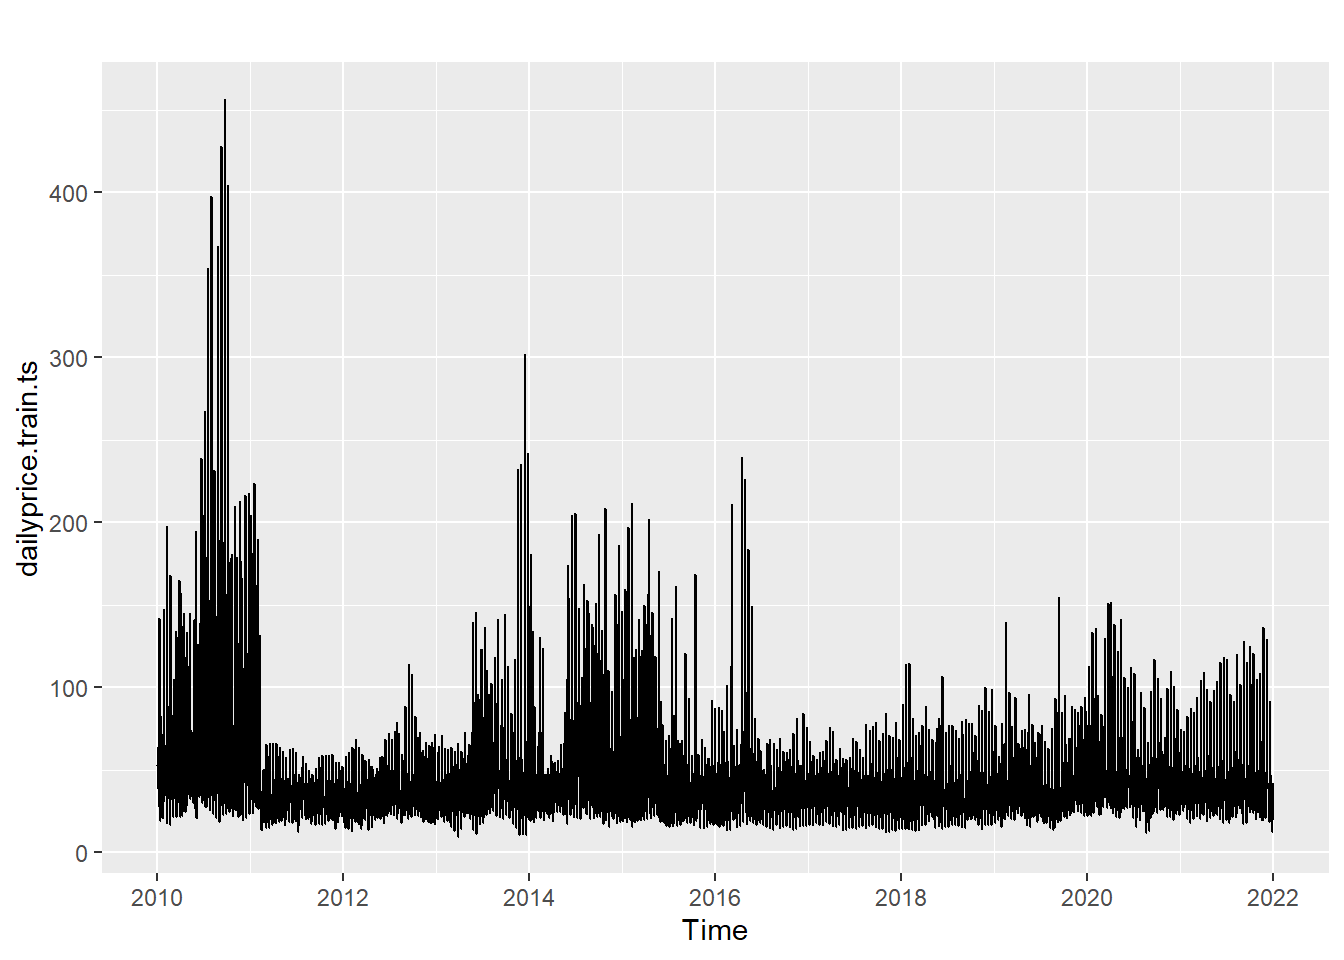
\includegraphics{TSA_Final_files/figure-latex/unnamed-chunk-6-1.pdf}

\begin{Shaded}
\begin{Highlighting}[]
\FunctionTok{autoplot}\NormalTok{ (dailyprice.test.ts)}
\end{Highlighting}
\end{Shaded}

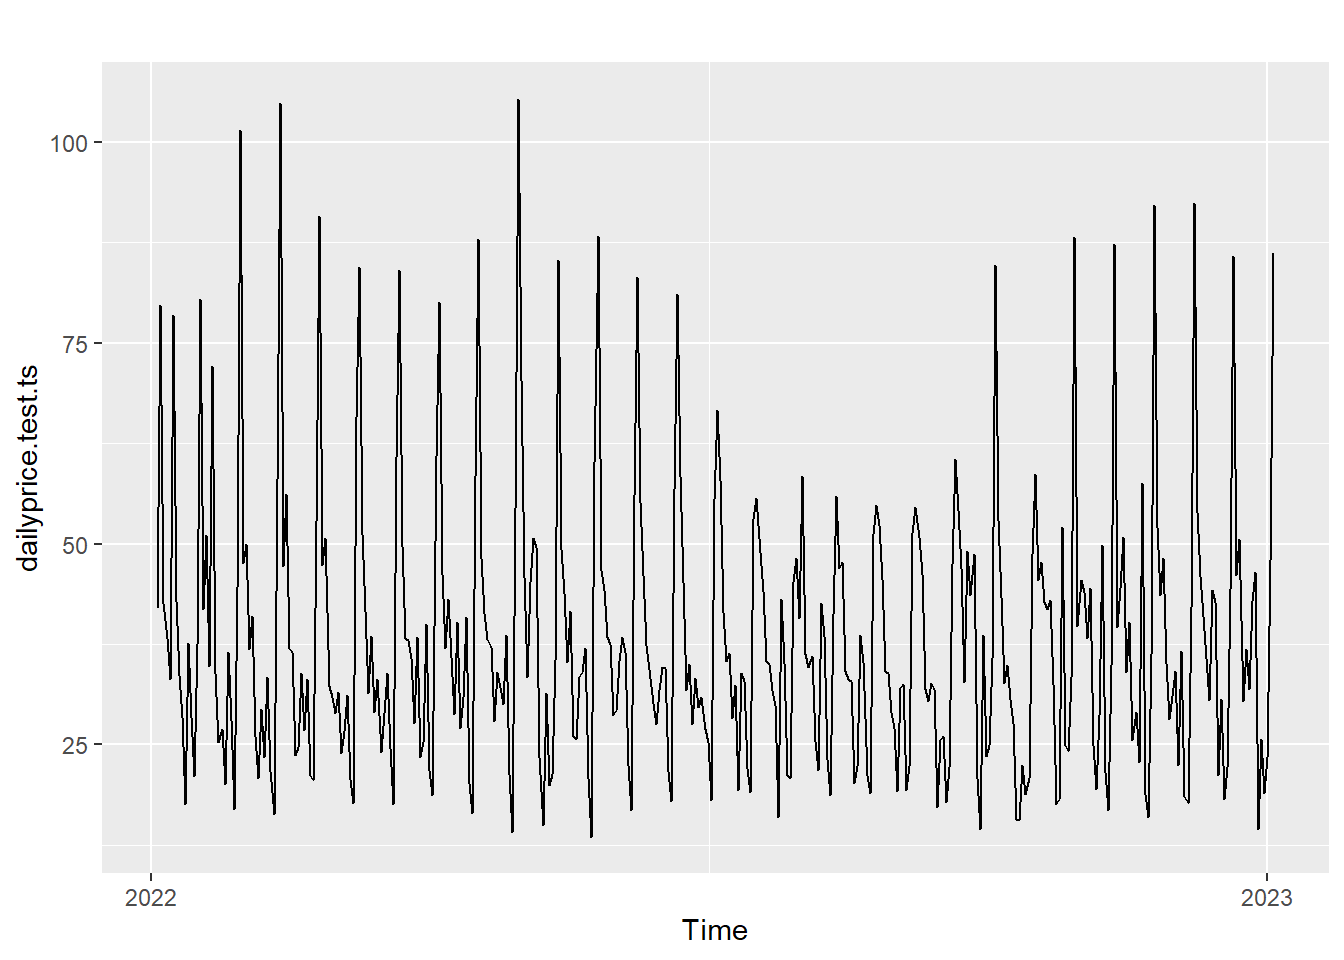
\includegraphics{TSA_Final_files/figure-latex/unnamed-chunk-6-2.pdf}

\begin{Shaded}
\begin{Highlighting}[]
\CommentTok{\# dailyload.ts \textless{}{-} msts(dailyload$daily\_mean\_load,}
\CommentTok{\#                       seasonal.periods = c(7,365.25),}
\CommentTok{\#                       start = c(2018,1,1)) }
\CommentTok{\# }
\CommentTok{\# NGprice.fixed.ts \textless{}{-} msts(NGprice.fixed$value,}
\CommentTok{\#                       seasonal.periods = c(7,365.25),}
\CommentTok{\#                       start = c(2018,1,1))}
\CommentTok{\# \#subsetting}
\CommentTok{\# dailyload.train.ts \textless{}{-} subset(dailyload.ts,}
\CommentTok{\#                                    end = length(dailyload.ts){-}365) \#Jan 1st 2018 to Dec 30st 2021}
\CommentTok{\# NGprice.fixed.train.ts \textless{}{-} subset(dailyload.ts,}
\CommentTok{\#                                    end = length(NGprice.fixed.ts){-}365) \#Jan 1st 2018 to Dec 31st 2021}
\end{Highlighting}
\end{Shaded}

\hypertarget{decomposing-time-series-objects}{%
\subsection{Decomposing time series
objects}\label{decomposing-time-series-objects}}

\begin{Shaded}
\begin{Highlighting}[]
\NormalTok{dailyprice.train.ts }\SpecialCharTok{\%\textgreater{}\%} \FunctionTok{mstl}\NormalTok{() }\SpecialCharTok{\%\textgreater{}\%} \FunctionTok{autoplot}\NormalTok{()}
\end{Highlighting}
\end{Shaded}

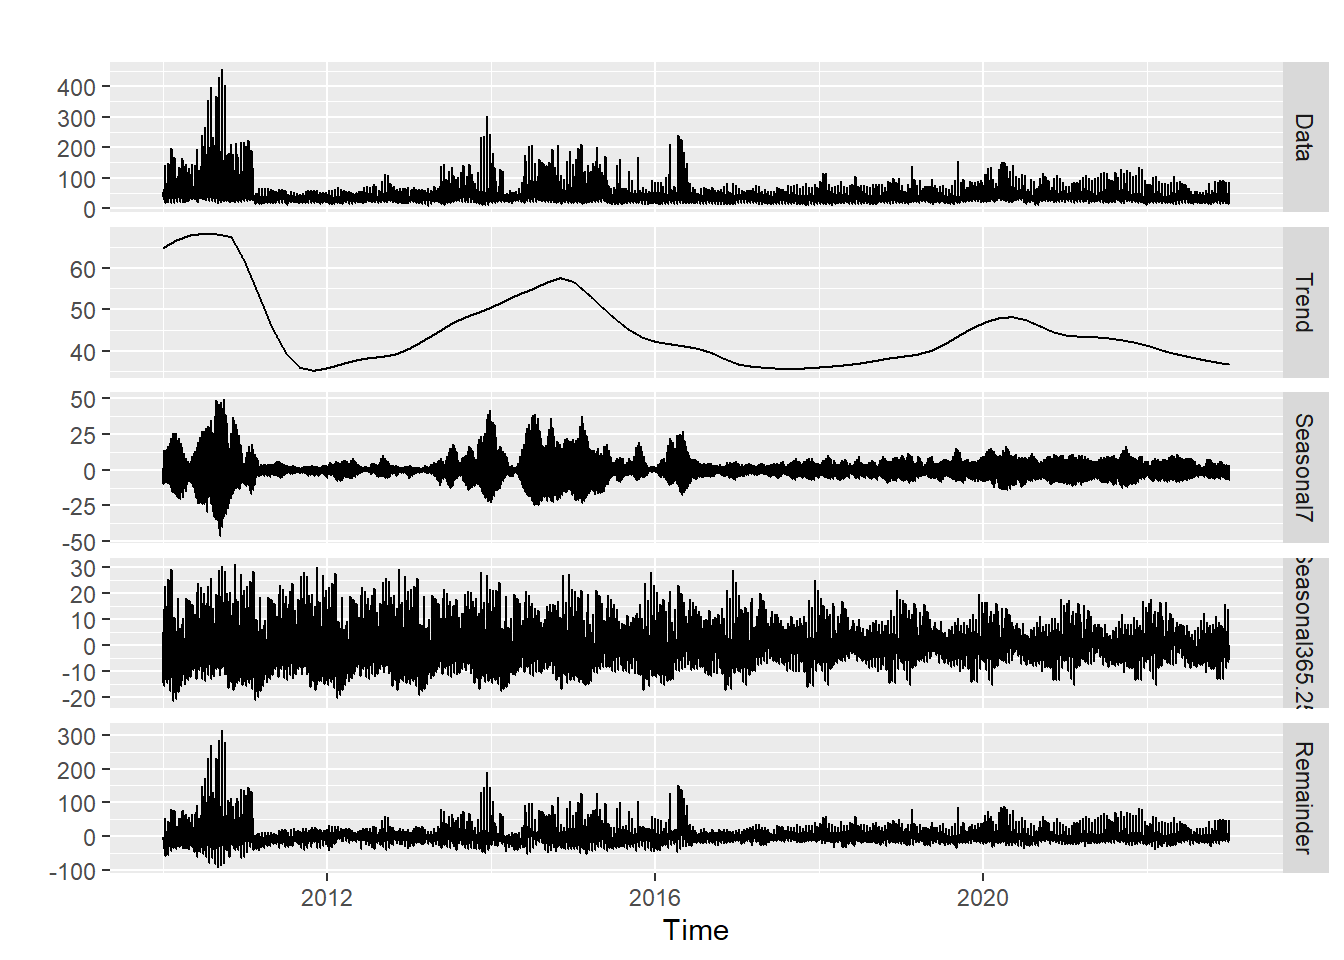
\includegraphics{TSA_Final_files/figure-latex/unnamed-chunk-7-1.pdf}

\hypertarget{exponential-smoothing-state-space-model}{%
\subsection{Exponential Smoothing State Space
Model}\label{exponential-smoothing-state-space-model}}

\begin{Shaded}
\begin{Highlighting}[]
\NormalTok{ETS\_fit }\OtherTok{\textless{}{-}}  \FunctionTok{stlf}\NormalTok{(dailyprice.train.ts, }\AttributeTok{h=}\DecValTok{365}\NormalTok{)}

\NormalTok{ETS\_plot}\OtherTok{\textless{}{-}}\FunctionTok{autoplot}\NormalTok{(dailyprice.test.ts, }\AttributeTok{color =} \StringTok{"dark grey"}\NormalTok{) }\SpecialCharTok{+}
  \FunctionTok{autolayer}\NormalTok{(ETS\_fit}\SpecialCharTok{$}\NormalTok{mean, }\AttributeTok{series=}\StringTok{"STL + ETS"}\NormalTok{,}\AttributeTok{PI=}\ConstantTok{FALSE}\NormalTok{, }\AttributeTok{color =} \StringTok{"blue"}\NormalTok{) }\SpecialCharTok{+}
  \FunctionTok{ylab}\NormalTok{(}\StringTok{"Electricity Price"}\NormalTok{)}
\end{Highlighting}
\end{Shaded}

\begin{verbatim}
## Warning in ggplot2::geom_line(ggplot2::aes_(x = ~timeVal, y = ~seriesVal, :
## Ignoring unknown parameters: `PI`
\end{verbatim}

\begin{Shaded}
\begin{Highlighting}[]
\NormalTok{ETS\_plot}
\end{Highlighting}
\end{Shaded}

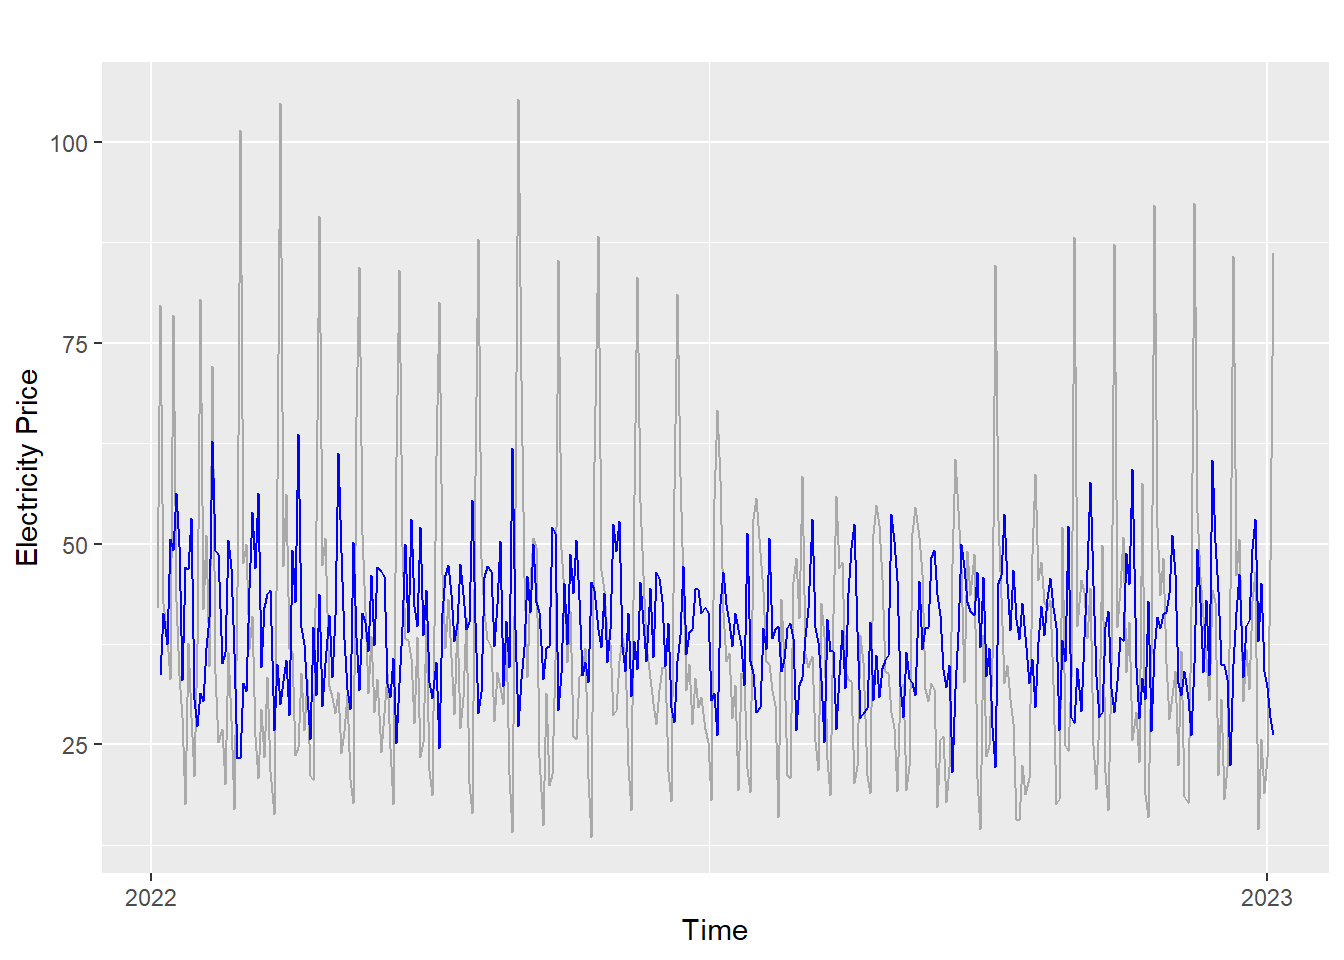
\includegraphics{TSA_Final_files/figure-latex/ETS Model-1.pdf}

\hypertarget{arima-with-dynamic-harmonic-fourier-components}{%
\subsection{ARIMA with dynamic harmonic fourier
components}\label{arima-with-dynamic-harmonic-fourier-components}}

\begin{Shaded}
\begin{Highlighting}[]
\NormalTok{ARIMA }\OtherTok{\textless{}{-}} \FunctionTok{auto.arima}\NormalTok{(dailyprice.train.ts,}
                  \AttributeTok{seasonal=}\ConstantTok{TRUE}\NormalTok{, }
                  \AttributeTok{lambda=}\DecValTok{0}\NormalTok{,}
                  \AttributeTok{xreg=}\FunctionTok{fourier}\NormalTok{(dailyprice.train.ts,}\AttributeTok{K=}\FunctionTok{c}\NormalTok{(}\DecValTok{2}\NormalTok{,}\DecValTok{12}\NormalTok{)))}
\CommentTok{\# ARIMA\_load \textless{}{-} auto.arima(dailyprice.train.ts,xreg=fourier(dailyload.train.ts,K=c(2,12)))}
\CommentTok{\# ARIMA\_ng\textless{}{-} auto.arima(dailyprice.train.ts,xreg=fourier(NGprice.fixed.train.ts,K=c(2,12)))}
\CommentTok{\# }
\CommentTok{\# dailyload.train.ts\_fc \textless{}{-} forecast(dailyload.train.ts,NGprice.fixed.train.ts, h = 365,level=0.9)}
\CommentTok{\# NGprice.fixed.train.ts\_fc \textless{}{-} forecast(dailyload.train.ts, h = 365)}

\NormalTok{ARIMA\_fc }\OtherTok{\textless{}{-}} \FunctionTok{forecast}\NormalTok{(ARIMA,}
                  \AttributeTok{xreg=}\FunctionTok{fourier}\NormalTok{(dailyprice.train.ts,}\AttributeTok{K=}\FunctionTok{c}\NormalTok{(}\DecValTok{2}\NormalTok{,}\DecValTok{12}\NormalTok{),}\AttributeTok{h=}\DecValTok{365}\NormalTok{),}\AttributeTok{h=}\DecValTok{365}\NormalTok{)}
\CommentTok{\# ARIMA\_load\_fc \textless{}{-} forecast(object = ARIMA\_origin\_fc,xreg=fourier(dailyload.train.ts\_fc$mean,K=c(2,12),h=365),h=365)}
\CommentTok{\# ARIMA\_ng\_fc \textless{}{-} forecast(object = ARIMA\_origin\_fc,xreg= fourier(NGprice.fixed.train.ts\_fc$mean,K=c(2,12),h=365),h=365)}

\CommentTok{\#Plot forecast with observed data}
\NormalTok{ARIMA\_plot }\OtherTok{\textless{}{-}} \FunctionTok{autoplot}\NormalTok{(dailyprice.test.ts, }\AttributeTok{color =} \StringTok{"dark grey"}\NormalTok{) }\SpecialCharTok{+}
  \FunctionTok{autolayer}\NormalTok{(ARIMA\_fc}\SpecialCharTok{$}\NormalTok{mean, }\AttributeTok{series=}\StringTok{"ARIMA\_xgre"}\NormalTok{,}\AttributeTok{PI=}\ConstantTok{FALSE}\NormalTok{,}\AttributeTok{color =} \StringTok{"blue"}\NormalTok{) }\SpecialCharTok{+}
  \FunctionTok{ylab}\NormalTok{(}\StringTok{"Electricity Price Forecast"}\NormalTok{)}
\end{Highlighting}
\end{Shaded}

\begin{verbatim}
## Warning in ggplot2::geom_line(ggplot2::aes_(x = ~timeVal, y = ~seriesVal, :
## Ignoring unknown parameters: `PI`
\end{verbatim}

\begin{Shaded}
\begin{Highlighting}[]
\NormalTok{ARIMA\_plot}
\end{Highlighting}
\end{Shaded}

\includegraphics{TSA_Final_files/figure-latex/ARIMA with dynamic harmonic fourier components-1.pdf}

\begin{Shaded}
\begin{Highlighting}[]
\CommentTok{\# }
\CommentTok{\# ARIMA\_load\_plot \textless{}{-} autoplot(dailyprice.test.ts, color = "dark grey") +}
\CommentTok{\#   autolayer(ARIMA\_load\_fc$mean, series="ARIMA\_xgre",PI=FALSE,color = "blue") +}
\CommentTok{\#   ylab("Electricity Price Forecast with EXO(load)")}
\CommentTok{\# ARIMA\_load\_plot }
\CommentTok{\# }
\CommentTok{\# ARIMA\_ng\_plot \textless{}{-}autoplot(dailyprice.test.ts, color = "dark grey") +}
\CommentTok{\#   autolayer(ARIMA\_ng\_fc$mean, series="ARIMA\_xgre",PI=FALSE,color = "blue") +}
\CommentTok{\#   ylab("Electricity Price Forecast with EXO(load)")}
\CommentTok{\# ARIMA\_ng\_plot}
\end{Highlighting}
\end{Shaded}

\hypertarget{tbats}{%
\subsection{TBATS}\label{tbats}}

\begin{Shaded}
\begin{Highlighting}[]
\NormalTok{TBATS\_fit }\OtherTok{\textless{}{-}} \FunctionTok{tbats}\NormalTok{(dailyprice.train.ts)}

\CommentTok{\#Forecast with TBATS}
\NormalTok{TBATS\_fc }\OtherTok{\textless{}{-}} \FunctionTok{forecast}\NormalTok{(TBATS\_fit, }\AttributeTok{h=}\DecValTok{365}\NormalTok{)}

\CommentTok{\#Plot forecast with observed data}
\FunctionTok{autoplot}\NormalTok{(dailyprice.test.ts, }\AttributeTok{color =} \StringTok{"dark grey"}\NormalTok{) }\SpecialCharTok{+}
  \FunctionTok{autolayer}\NormalTok{(TBATS\_fc}\SpecialCharTok{$}\NormalTok{mean, }\AttributeTok{series=}\StringTok{"TBATS"}\NormalTok{,}\AttributeTok{PI=}\ConstantTok{FALSE}\NormalTok{, }\AttributeTok{color =} \StringTok{"blue"}\NormalTok{)}\SpecialCharTok{+}
  \FunctionTok{ylab}\NormalTok{(}\StringTok{"Electricity Price"}\NormalTok{)}
\end{Highlighting}
\end{Shaded}

\begin{verbatim}
## Warning in ggplot2::geom_line(ggplot2::aes_(x = ~timeVal, y = ~seriesVal, :
## Ignoring unknown parameters: `PI`
\end{verbatim}

\includegraphics{TSA_Final_files/figure-latex/TBATS-1.pdf}

\hypertarget{neural-network}{%
\subsection{Neural Network}\label{neural-network}}

\begin{Shaded}
\begin{Highlighting}[]
\NormalTok{NN\_origin }\OtherTok{\textless{}{-}} \FunctionTok{nnetar}\NormalTok{(dailyprice.train.ts,}\AttributeTok{p=}\DecValTok{1}\NormalTok{,}\AttributeTok{P=}\DecValTok{0}\NormalTok{,}\AttributeTok{xreg=}\FunctionTok{fourier}\NormalTok{(dailyprice.train.ts, }\AttributeTok{K=}\FunctionTok{c}\NormalTok{(}\DecValTok{2}\NormalTok{,}\DecValTok{12}\NormalTok{)))}
\CommentTok{\#NN\_load \textless{}{-} nnetar(dailyprice.train.ts,p=1,P=0,xreg=fourier(dailyload.train.ts,K=c(2,12)))}
\CommentTok{\#NN\_ng \textless{}{-} nnetar(dailyprice.train.ts,p=1,P=0,xreg=fourier(NGprice.fixed.train.ts,K=c(2,12)))}


\CommentTok{\#Forecast with NNet}
\NormalTok{NN\_origin\_fc}\OtherTok{\textless{}{-}} \FunctionTok{forecast}\NormalTok{(NN\_origin,}\AttributeTok{h=}\DecValTok{365}\NormalTok{,}\AttributeTok{xreg=}\FunctionTok{fourier}\NormalTok{(dailyprice.train.ts,}\AttributeTok{K=}\FunctionTok{c}\NormalTok{(}\DecValTok{2}\NormalTok{,}\DecValTok{12}\NormalTok{),}\AttributeTok{h=}\DecValTok{365}\NormalTok{))}
\CommentTok{\#NN\_load\_fc \textless{}{-} forecast(NN\_load, h=365,xreg=fourier(dailyload.train.ts\_fc$mean,K=c(2,12)))}
\CommentTok{\#NN\_ng\_fc \textless{}{-}forecast(NN\_ng, h=365,xreg=fourier(NGprice.fixed.train.ts,K=c(2,12)))}

\CommentTok{\#Plot forecast with observed data}
\FunctionTok{autoplot}\NormalTok{(dailyprice.test.ts, }\AttributeTok{color =} \StringTok{"dark grey"}\NormalTok{) }\SpecialCharTok{+}
  \FunctionTok{autolayer}\NormalTok{(NN\_origin\_fc}\SpecialCharTok{$}\NormalTok{mean, }\AttributeTok{series=}\StringTok{"Neural Network"}\NormalTok{,}\AttributeTok{PI=}\ConstantTok{FALSE}\NormalTok{, }\AttributeTok{color =} \StringTok{"blue"}\NormalTok{)}\SpecialCharTok{+}
  \FunctionTok{ylab}\NormalTok{(}\StringTok{"Electricity Price"}\NormalTok{) }
\end{Highlighting}
\end{Shaded}

\begin{verbatim}
## Warning in ggplot2::geom_line(ggplot2::aes_(x = ~timeVal, y = ~seriesVal, :
## Ignoring unknown parameters: `PI`
\end{verbatim}

\includegraphics{TSA_Final_files/figure-latex/Neural Network-1.pdf}

\begin{Shaded}
\begin{Highlighting}[]
\CommentTok{\# NN\_load\_plot \textless{}{-} autoplot(dailyprice.test.ts, color = "dark grey") +}
\CommentTok{\#   autolayer(NN\_load\_fc$mean, series="Neural Network",PI=FALSE, color = "blue")+}
\CommentTok{\#   ylab("Electricity Price") }
\CommentTok{\# NN\_load\_plot}
\CommentTok{\# }
\CommentTok{\# NN\_ng\_plot \textless{}{-} autoplot(dailyprice.test.ts, color = "dark grey") +}
\CommentTok{\#   autolayer(NN\_ng\_fc$mean, series="Neural Network",PI=FALSE, color = "blue")+}
\CommentTok{\#   ylab("Electricity Price") }
\CommentTok{\# NN\_ng\_plot}
\end{Highlighting}
\end{Shaded}

\hypertarget{checking-accuracy-of-models}{%
\subsection{Checking accuracy of
models}\label{checking-accuracy-of-models}}

\begin{Shaded}
\begin{Highlighting}[]
\CommentTok{\#Model 1: STL + ETS}
\NormalTok{ETS\_score }\OtherTok{\textless{}{-}} \FunctionTok{accuracy}\NormalTok{(ETS\_fit}\SpecialCharTok{$}\NormalTok{mean, dailyprice.test.ts)  }
\CommentTok{\#Model 2: ARIMA }
\NormalTok{ARIMA\_score }\OtherTok{\textless{}{-}} \FunctionTok{accuracy}\NormalTok{(ARIMA\_fc}\SpecialCharTok{$}\NormalTok{mean, dailyprice.test.ts)}
\CommentTok{\# \#Model 2.1: ARIMA + Fourier(Load)}
\CommentTok{\# ARIMA\_load\_score \textless{}{-} accuracy(ARIMA\_load\_fc$mean, dailyprice.test.ts)}
\CommentTok{\# \#Model 2.2: ARIMA + Fourier(NG)}
\CommentTok{\# ARIMA\_ng\_score \textless{}{-} accuracy(ARIMA\_ng\_fc$mean, dailyprice.test.ts)}

\CommentTok{\# Model 3:  TBATS }
\NormalTok{TBATS\_score }\OtherTok{\textless{}{-}} \FunctionTok{accuracy}\NormalTok{(TBATS\_fc}\SpecialCharTok{$}\NormalTok{mean, dailyprice.test.ts)}
\CommentTok{\# Model 4:  Neural Network }
\NormalTok{NN\_score }\OtherTok{\textless{}{-}} \FunctionTok{accuracy}\NormalTok{(NN\_origin\_fc}\SpecialCharTok{$}\NormalTok{mean, dailyprice.test.ts)}
\CommentTok{\# \# Model 4.1:  Neural Network }
\CommentTok{\# NN\_load\_score \textless{}{-} accuracy(NN\_load\_fc$mean, dailyprice.test.ts)}
\CommentTok{\# \# Model 4.2:  Neural Network }
\CommentTok{\# NN\_ng\_score \textless{}{-} accuracy(NN\_ng\_fc$mean, dailyprice.test.ts)}
\end{Highlighting}
\end{Shaded}

\hypertarget{compare-performance-metrics}{%
\subsection{Compare performance
metrics}\label{compare-performance-metrics}}

\begin{Shaded}
\begin{Highlighting}[]
\CommentTok{\#create data frame}
\NormalTok{scores }\OtherTok{\textless{}{-}} \FunctionTok{as.data.frame}\NormalTok{(}
  \FunctionTok{rbind}\NormalTok{(ETS\_score, ARIMA\_score, TBATS\_score, NN\_score)}
\NormalTok{  )}
\FunctionTok{row.names}\NormalTok{(scores) }\OtherTok{\textless{}{-}} \FunctionTok{c}\NormalTok{(}\StringTok{"ETS"}\NormalTok{, }\StringTok{"ARIMA"}\NormalTok{,}\StringTok{"TBATS"}\NormalTok{, }\StringTok{"NN"}\NormalTok{)}

\CommentTok{\# scores \textless{}{-} as.data.frame(}
\CommentTok{\#   rbind(ETS\_score, ARIMA\_score,ARIMA\_load\_score,ARIMA\_ng\_score, TBATS\_score, NN\_score,NN\_load\_score, NN\_load\_score)}
\CommentTok{\#   )}
\CommentTok{\# row.names(scores) \textless{}{-} c("ETS", "ARIMA","ARIMA + exo(load)" ,"ARIMA + exo(ng)","TBATS", "NN", "NN+ exo(load)", "NN+ exo(ng)")}
\CommentTok{\#choose model with lowest RMSE}
\NormalTok{best\_model\_index }\OtherTok{\textless{}{-}} \FunctionTok{which.min}\NormalTok{(scores[,}\StringTok{"RMSE"}\NormalTok{])}
\FunctionTok{cat}\NormalTok{(}\StringTok{"The best model by RMSE is:"}\NormalTok{, }\FunctionTok{row.names}\NormalTok{(scores[best\_model\_index,]))                       }
\end{Highlighting}
\end{Shaded}

\begin{verbatim}
## The best model by RMSE is: ARIMA
\end{verbatim}

\begin{Shaded}
\begin{Highlighting}[]
\FunctionTok{kbl}\NormalTok{(scores, }
      \AttributeTok{caption =} \StringTok{"Forecast Accuracy for Electricity Price"}\NormalTok{,}
      \AttributeTok{digits =} \FunctionTok{array}\NormalTok{(}\DecValTok{5}\NormalTok{,}\FunctionTok{ncol}\NormalTok{(scores))) }\SpecialCharTok{\%\textgreater{}\%}
  \FunctionTok{kable\_styling}\NormalTok{(}\AttributeTok{full\_width =} \ConstantTok{FALSE}\NormalTok{, }\AttributeTok{position =} \StringTok{"center"}\NormalTok{, }\AttributeTok{latex\_options =} \StringTok{"hold\_position"}\NormalTok{) }\SpecialCharTok{\%\textgreater{}\%}
  \CommentTok{\#highlight model with lowest RMSE}
  \FunctionTok{kable\_styling}\NormalTok{(}\AttributeTok{latex\_options=}\StringTok{"striped"}\NormalTok{, }\AttributeTok{stripe\_index =} \FunctionTok{which.min}\NormalTok{(scores[,}\StringTok{"RMSE"}\NormalTok{]))}
\end{Highlighting}
\end{Shaded}

\begin{table}[!h]

\caption{\label{tab:unnamed-chunk-10}Forecast Accuracy for Electricity Price}
\centering
\begin{tabular}[t]{l|r|r|r|r|r|r|r}
\hline
  & ME & RMSE & MAE & MPE & MAPE & ACF1 & Theil's U\\
\hline
ETS & -1.06882 & 20.59728 & 15.63560 & -23.91673 & 47.02534 & 0.40019 & 0.98470\\
\hline
\cellcolor{gray!6}{ARIMA} & \cellcolor{gray!6}{0.62379} & \cellcolor{gray!6}{17.25831} & \cellcolor{gray!6}{12.67810} & \cellcolor{gray!6}{-17.28693} & \cellcolor{gray!6}{38.19677} & \cellcolor{gray!6}{0.36860} & \cellcolor{gray!6}{0.81055}\\
\hline
TBATS & 1.18936 & 17.26567 & 12.55564 & -15.54596 & 37.34337 & 0.37153 & 0.80490\\
\hline
NN & -8.46039 & 21.10422 & 16.27590 & -45.52954 & 58.05176 & 0.26333 & 1.19713\\
\hline
\end{tabular}
\end{table}

\begin{Shaded}
\begin{Highlighting}[]
\FunctionTok{autoplot}\NormalTok{(dailyprice.test.ts) }\SpecialCharTok{+}
  \FunctionTok{autolayer}\NormalTok{(ETS\_fit, }\AttributeTok{PI=}\ConstantTok{FALSE}\NormalTok{, }\AttributeTok{series=}\StringTok{"STL+ETS"}\NormalTok{) }\SpecialCharTok{+}
  \FunctionTok{autolayer}\NormalTok{(ARIMA\_fc, }\AttributeTok{PI=}\ConstantTok{FALSE}\NormalTok{, }\AttributeTok{series=}\StringTok{"ARIMA"}\NormalTok{) }\SpecialCharTok{+}
  \FunctionTok{autolayer}\NormalTok{(TBATS\_fc,}\AttributeTok{PI=}\ConstantTok{FALSE}\NormalTok{, }\AttributeTok{series=}\StringTok{"TBATS"}\NormalTok{) }\SpecialCharTok{+}
  \FunctionTok{autolayer}\NormalTok{(NN\_origin\_fc,}\AttributeTok{PI=}\ConstantTok{FALSE}\NormalTok{, }\AttributeTok{series=}\StringTok{"NN"}\NormalTok{) }\SpecialCharTok{+}
  \FunctionTok{xlab}\NormalTok{(}\StringTok{"Day"}\NormalTok{) }\SpecialCharTok{+} \FunctionTok{ylab}\NormalTok{(}\StringTok{"Electricity Price"}\NormalTok{) }\SpecialCharTok{+}
  \FunctionTok{guides}\NormalTok{(}\AttributeTok{colour=}\FunctionTok{guide\_legend}\NormalTok{(}\AttributeTok{title=}\StringTok{"Forecast"}\NormalTok{))}
\end{Highlighting}
\end{Shaded}

\includegraphics{TSA_Final_files/figure-latex/unnamed-chunk-11-1.pdf}

\hypertarget{predicting-the-future}{%
\subsection{Predicting the future}\label{predicting-the-future}}

\begin{Shaded}
\begin{Highlighting}[]
\NormalTok{ETS\_fit\_2023 }\OtherTok{\textless{}{-}}  \FunctionTok{stlf}\NormalTok{(dailyprice.ts, }\AttributeTok{h=}\DecValTok{365}\NormalTok{)}

\FunctionTok{autoplot}\NormalTok{(dailyprice.test.ts, }\AttributeTok{color =} \StringTok{"dark grey"}\NormalTok{) }\SpecialCharTok{+}
  \FunctionTok{autolayer}\NormalTok{(ETS\_fit\_2023}\SpecialCharTok{$}\NormalTok{mean, }\AttributeTok{series=}\StringTok{"STL + ETS"}\NormalTok{,}\AttributeTok{PI=}\ConstantTok{FALSE}\NormalTok{, }\AttributeTok{color =} \StringTok{"blue"}\NormalTok{) }\SpecialCharTok{+}
  \FunctionTok{ylab}\NormalTok{(}\StringTok{"Electricity Price"}\NormalTok{)}
\end{Highlighting}
\end{Shaded}

\begin{verbatim}
## Warning in ggplot2::geom_line(ggplot2::aes_(x = ~timeVal, y = ~seriesVal, :
## Ignoring unknown parameters: `PI`
\end{verbatim}

\includegraphics{TSA_Final_files/figure-latex/unnamed-chunk-12-1.pdf}

\end{document}
